\documentclass[10pt,a4paper]{article}
\usepackage[utf8]{inputenc}
%\usepackage[french]{babel}
\usepackage{tikz-network}
\usepackage{tikz}
\usepackage{graphics,multirow}
\usepackage{subcaption}
\usepackage{array}
\usepackage{xcolor}
\PassOptionsToPackage{hyphens}{url}
\usepackage{hyperref}
\usepackage{amsmath}
\usepackage{amsfonts}
\usepackage{amssymb}
\usepackage{mathtools}
\usepackage[total={6in,8in}]{geometry}
\usepackage[backend=biber,style=numeric,sorting=ynt]{biblatex}
\newcommand{\red}[1]{{\textcolor{red}{#1}}}
\newcommand{\green}[1]{{\textcolor{green}{#1}}}
\newcommand{\orange}[1]{{\textcolor{orange}{#1}}}
\addbibresource{report.bib}
 \hypersetup{
 %   bookmarks=true,         % show bookmarks bar?
 %   unicode=false,          % non-Latin characters in Acrobat’s bookmarks
 %   pdftoolbar=true,        % show Acrobat’s toolbar?
 %   pdfmenubar=true,        % show Acrobat’s menu?
 %   pdffitwindow=false,     % window fit to page when opened
 %   pdfstartview={FitH},    % fits the width of the page to the window
 %   pdftitle={My title},    % title
 %   pdfauthor={Author},     % author
 %   pdfsubject={Subject},   % subject of the document
 %   pdfcreator={Creator},   % creator of the document
 %   pdfproducer={Producer}, % producer of the document
 %   pdfkeywords={keyword1, key2, key3}, % list of keywords
 %   pdfnewwindow=true,      % links in new PDF window
    colorlinks=true,       % false: boxed links; true: colored links
    linkcolor=blue,          % color of internal links (change box color with linkbordercolor)
    citecolor=blue,        % color of links to bibliography
    filecolor=blue,         % color of file links
    urlcolor=blue        % color of external links
}
%% COLORS %%
%
\definecolor{mygreen}{RGB}{0,214,0}
%% MACROS %%

\newcommand\von{{\textsc{Von}}}
\newcommand\fon{{\textsc{Fon}}}
\newcommand\hon{{\textsc{Hon}}}
\newcommand\fston{$1^{\mathrm{st}}${\textsc{on}}}
\newcommand\nrep{N_{\mathrm{rep}}}
\newcommand\uprvec{\Pi_{\mathrm{Von}}^{\mathrm{U}}}
\newcommand\bprvec{\Pi_{\mathrm{1}}^{\mathrm{B}}}
\newcommand\hprvec{\Pi_{\mathrm{Von}}}
\newcommand\fprvec{\Pi_{\mathrm{1}}}
\newcommand\urank{K_{\mathrm{Von}}^{\mathrm{U}}}
\newcommand\brank{K_{\mathrm{1}}^{\mathrm{B}}}
\newcommand\hrank{K_{\mathrm{Von}}}
\newcommand\frank{K_{\mathrm{1}}}
\newcommand\vrank{K_{\mathrm{V}}}
\newcommand\reprank{K_{\mathrm{rep}}}
\newcommand{\tbd}[1]{\textcolor{blue}{{\textbf{To do: #1}}}}
\newcommand{\ask}[1]{\textcolor{red}{{\textbf{Question: #1}}}}
\newcommand\mems{\textit{memory nodes}}
\newcommand\kin{k_{\mathrm{in}}}
\newcommand\kout{k_{\mathrm{out}}}
\newcommand\uhonpr{Unbiased HON PR}
\newcommand\honpr{HON PR}
\newcommand\pr{1stON PR}
\newcommand\bpr{1stON Biased PR}
%\author{Célestin Coquidé}
\title{Complexity and Fitness of Methylated DNA sites and RNAs in the context of Breast Cancer Tissues}
\date{\today}
\begin{document}
\maketitle
\section{Aim of the study}
Highlighting the nestedness structure of the bipartite network representing correlations between methylated DNA sited and RNAs.
\section{Methods and Data}
\subsection{Nestedness}
Nested structures appear in the nature such that in ecological and socio-economic systems. In ecological systems, for instance, there is a nested distribution of species habitats. Where as some species only live in particular locations, some others live in a large variety of environments including those particular locations. In the context of network theory, a perfectly nested structure is such that for any pair of node ($i,j$) with $k_{i} < k_{j}$ their respective degree (number of neighbors), the set of nodes $i$ is interacting with is included in the set of nodes $j$ is interacting with. The adjacency matrix of such a network shows a triangular shape when columns and rows are sorted accordingly to the degree ordering of respective nodes. There are many metrics (other than degrees) permitting to infer the nested structure of a given network. Nestedness can appear in unipartite and bipartite networks. In the context of economical systems, especially the world trade network seen as a country-product bipartite network, recent research shows the existence of nestedness, see a complete review in \cite{mariani19}. In the context of biological systems nestedness structures have also been studied. In \cite{cantor17} different biological scales are considered. However, it seems that DNA-RNA interactions have not been studied yet. We choose the metric called fitness-complexity introduced in \cite{tacchella12} to investigate the nestedness structure of DNA-RNA bipartite network. Fitness and complexity is a non-linear and iterative algorithm permitting to infer the nestedness in bipartite network such as economical networks. In this context, the fitness is a country quality, and complexity is a product quality. In our approach we try to make an analogy where RNAs play the role of products and DNAs the role of countries. Here are the economical definitions of fitness and complexity.
\paragraph{Country's fitness}
\paragraph{Product's complexity}
\subsection{Data}
We used an open access cancer dataset from GDC Data Portal. From raw data consisting in methylated DNA and RNA's beta-values for up to 841 tumorous and normal breast tissues, we built a Matrix of Pearson Correlation Coefficients between Methylated DNA and RNA from these beta-values. A network representing the Pearson correlation coefficients between pairs (M-DNA,RNA) consists in a bipartite graph with coefficients as weight of the links. Two possibilities are considered either the correlation is positive or negative. Therefore we consider a signed bipartite graph with undirected links. Two other correlation matrices can be constructed from these beta-values, the DNA-DNA and RNA-RNA correlation matrices.

We are doing an analogy with the fitness-complexity nestedness model proposed in [citation] where DNAs and RNAs are treated as countries and products.
\section{The case of ESR1 synthesis and regulation}
Here is presented some preliminary results obtained by performing fitness-complexity model on a subset of the dataset. We are considering 508 RNAs and 13707 DNAs involved in ESR1 synthesis and regulation. We can see that, for different Pearson correlation thresholds, both positive and negative Pearson correlations based interactions between DNAs and RNAs, from this subset, present a nested structure.
\begin{figure}[h!]
\resizebox{\columnwidth}{!}{%
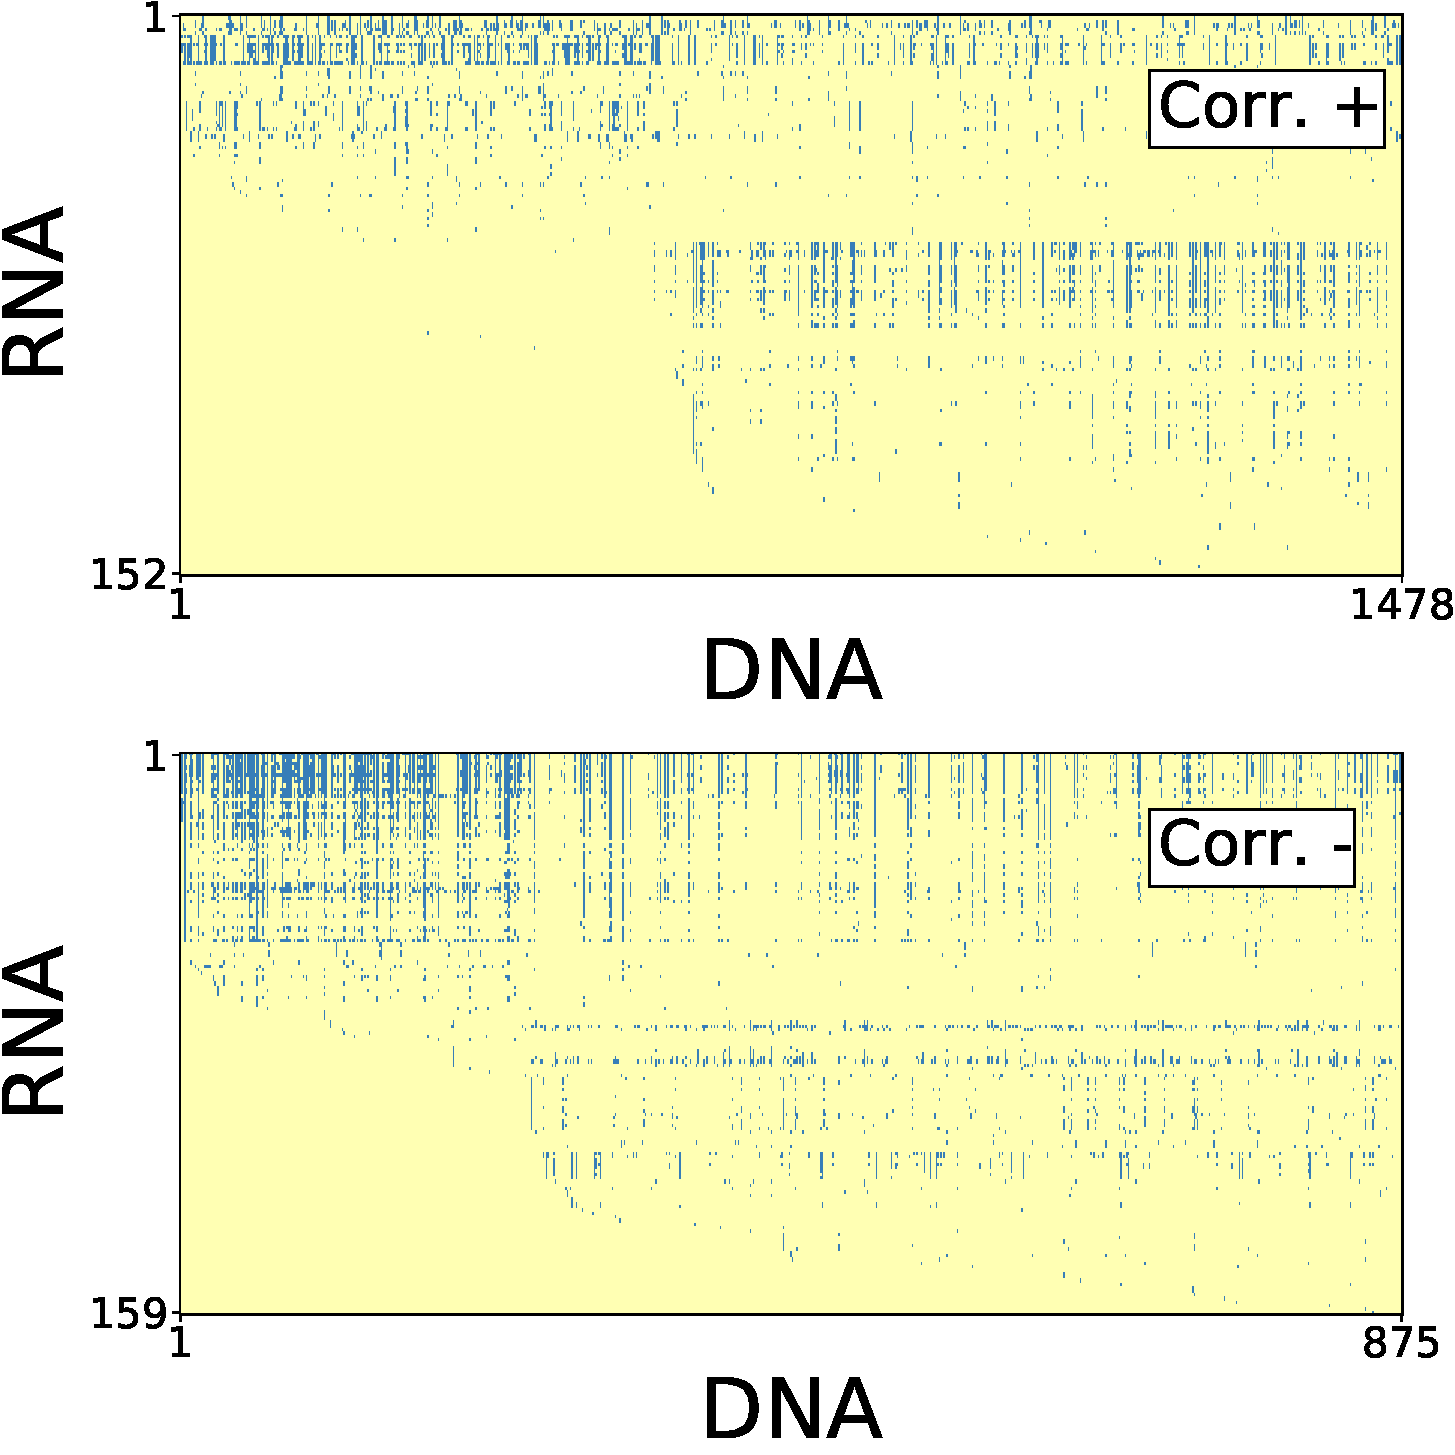
\includegraphics[width=\columnwidth]{FIG/ADN-ARN_Matrix-unit-0.5.pdf}
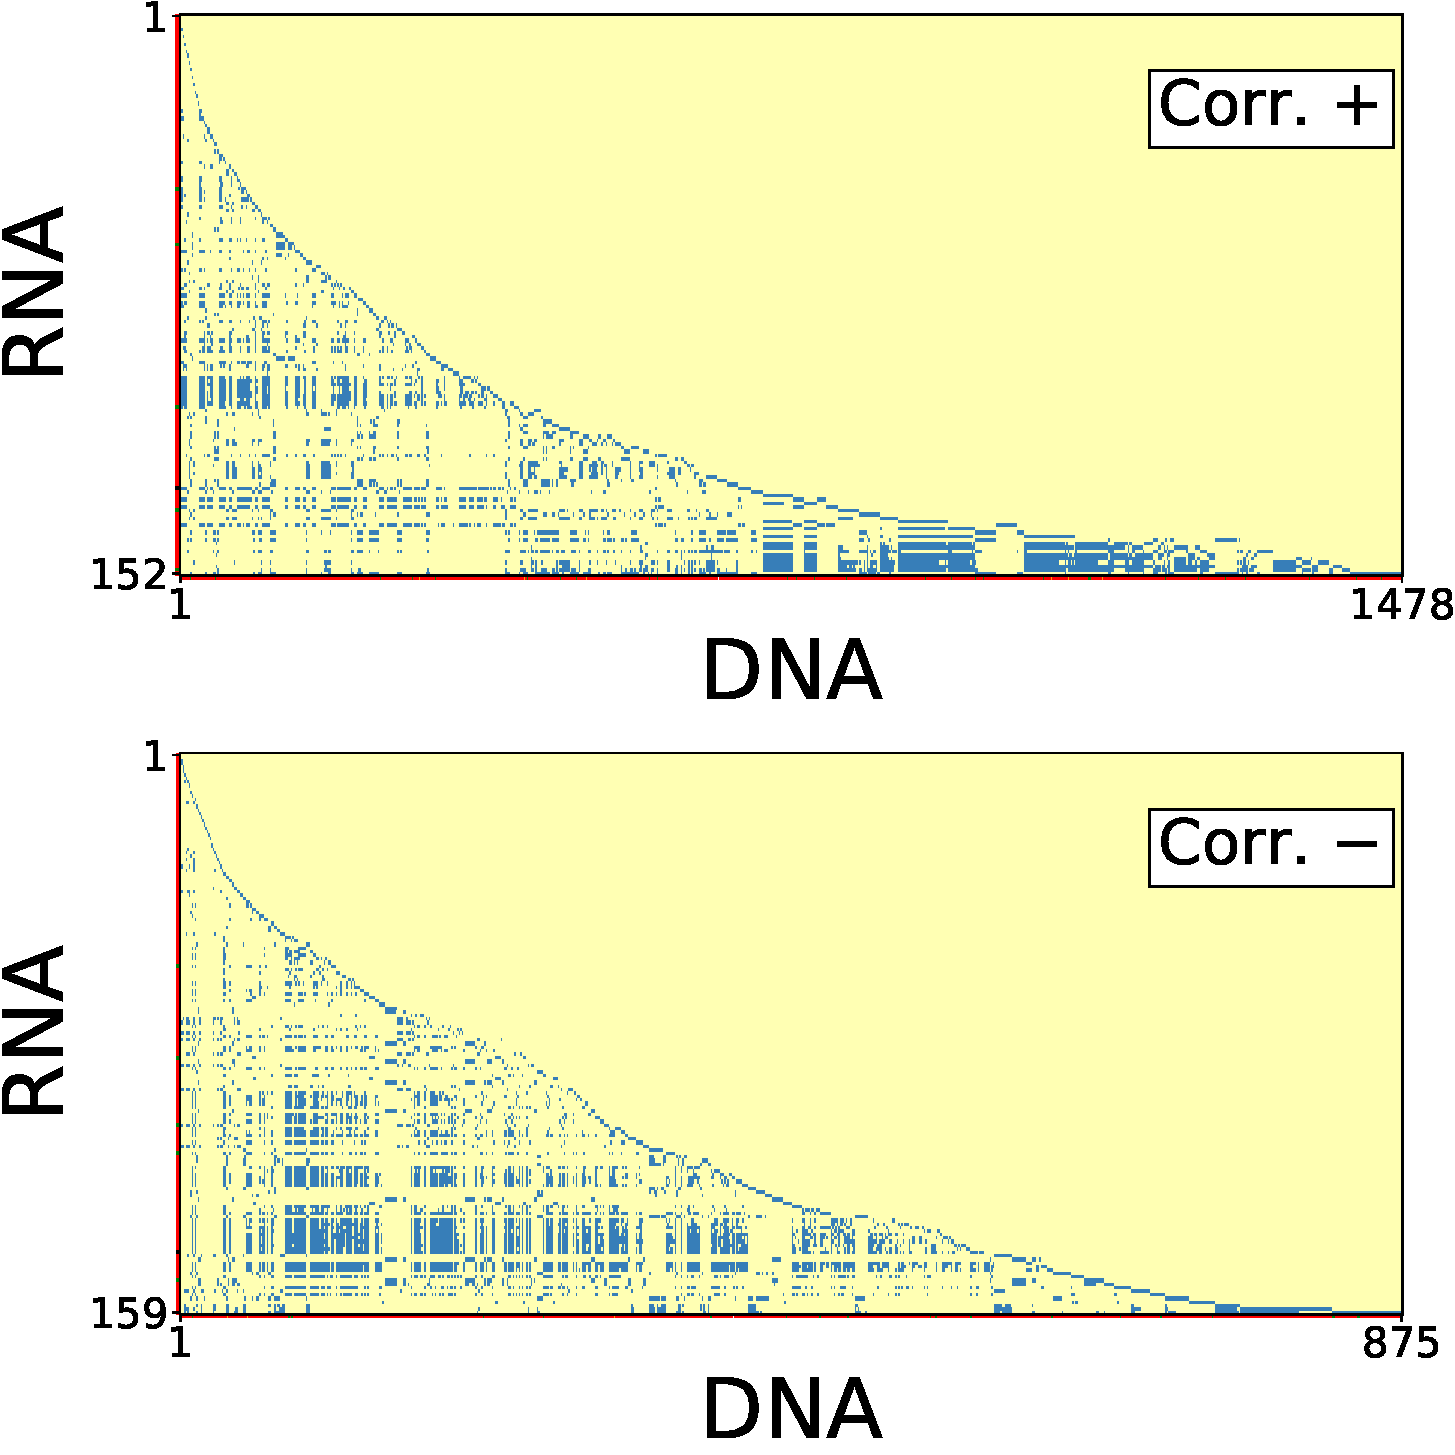
\includegraphics[width=\columnwidth]{FIG/ADN-ARN_FQ-Matrix-sum-unit-0.5.pdf}
}
\begin{center}
\vspace{-2pt}
\rule{\textwidth}{2pt}
\end{center}
\resizebox{\columnwidth}{!}{%
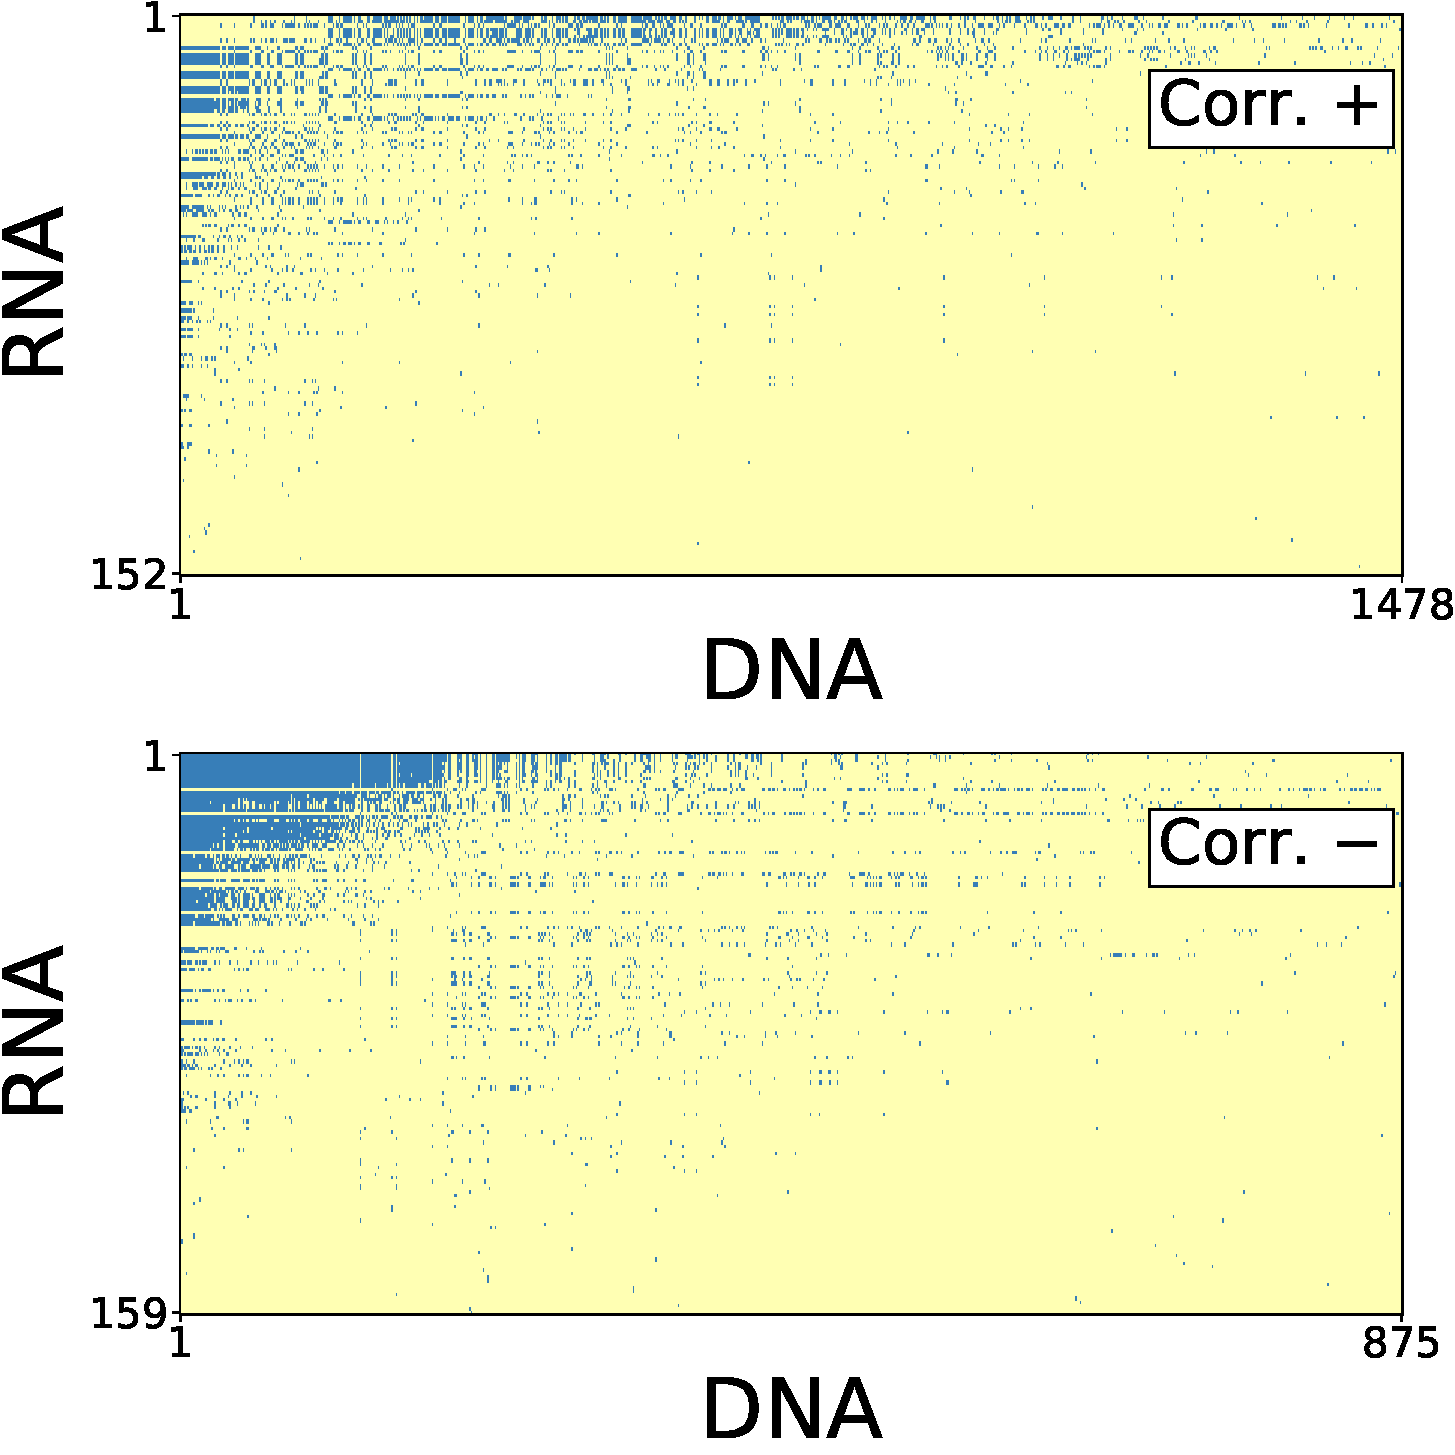
\includegraphics[width=\columnwidth]{FIG/ADN-ARN_Degree-Matrix-unit-0.5.pdf}
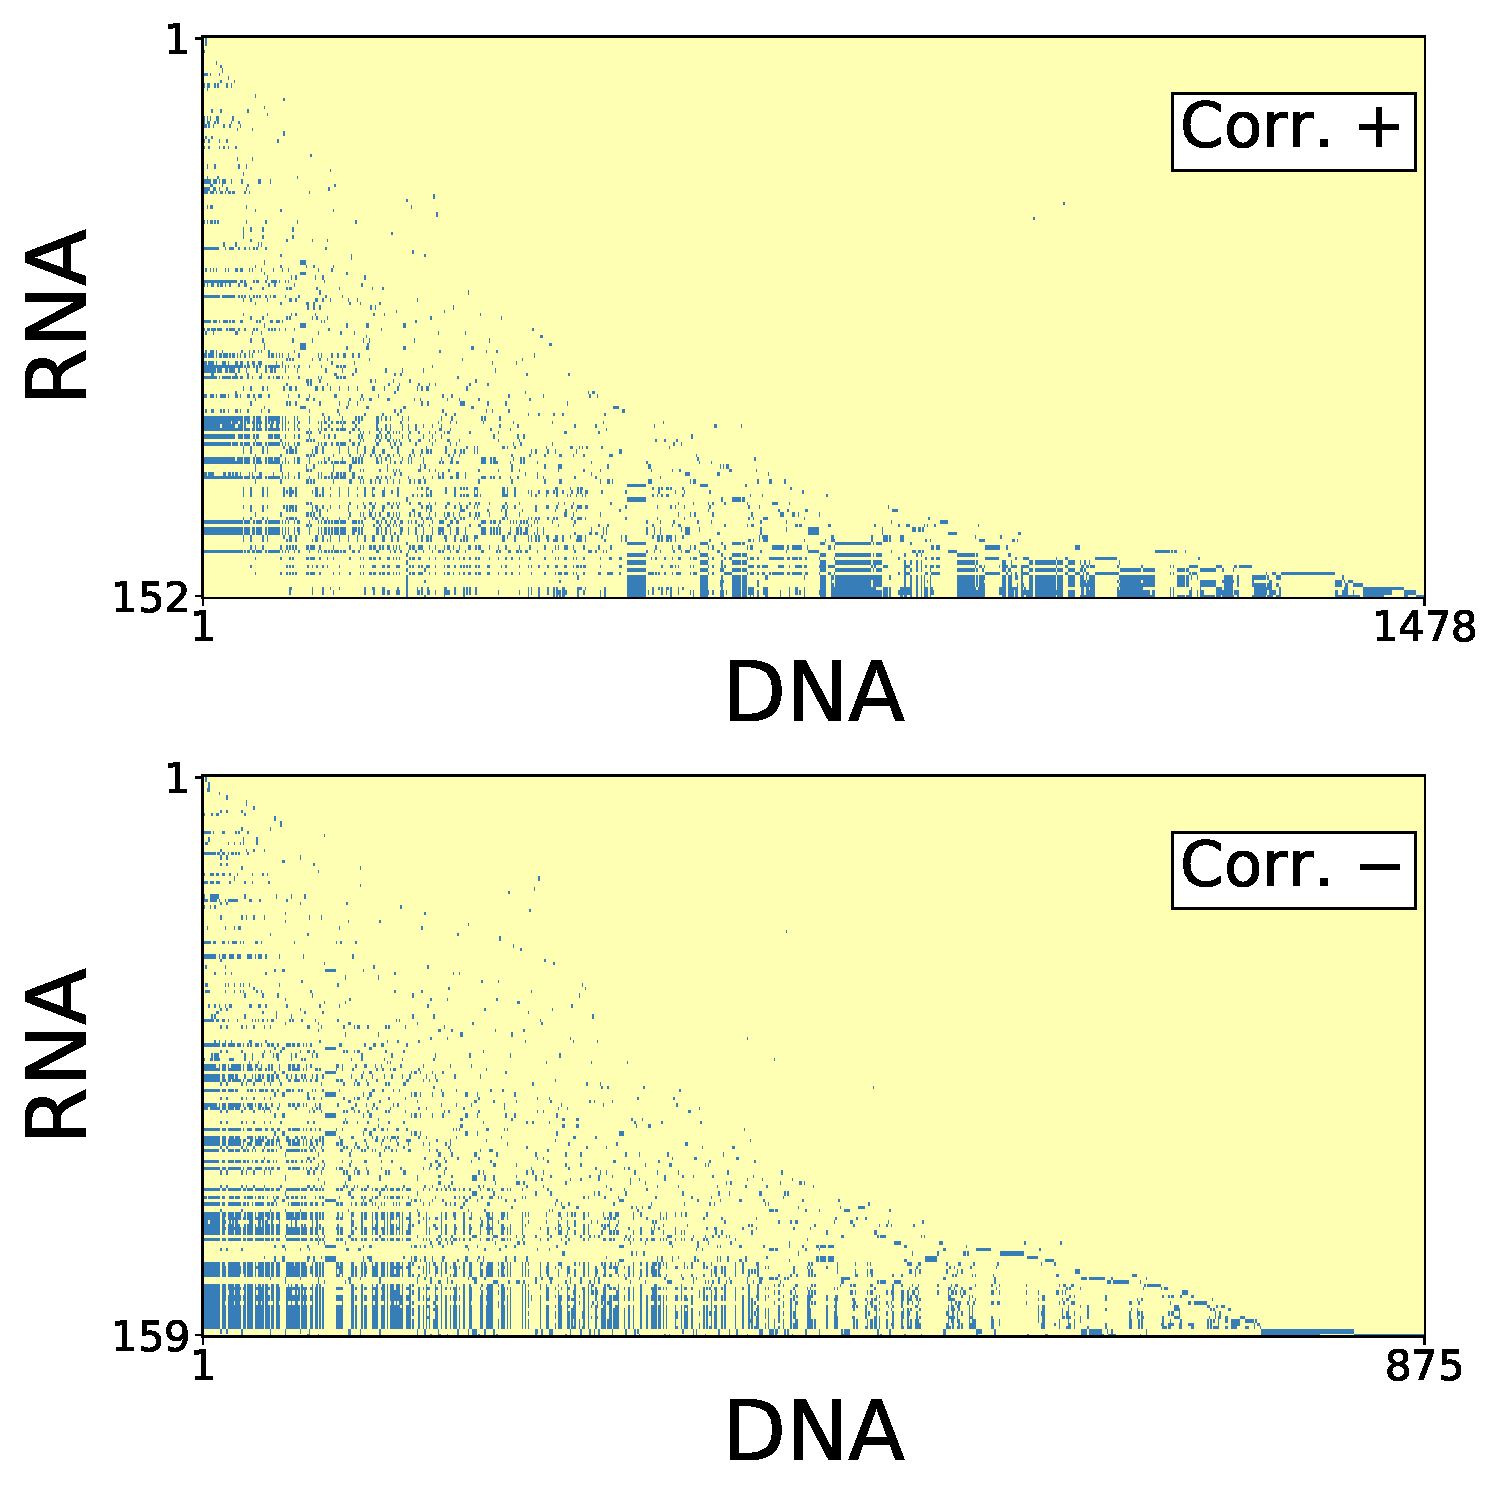
\includegraphics[width=\columnwidth]{FIG/ADN_ARN_BINMATNEST-Matrix-unit-0.5.pdf}
}
\caption{\label{fig:fig1}Binary bi-adjacency matrix representing the interactions between DNAs and RNAs involved in ESR1 synthesis and regulation. Matrix entries equal to $1$ (blue cells) if there is an interaction between entities, $0$ otherwise (bright yellow cells). Raw matrix (top left), Fitness and Complexity based reorganized matrix (top right), Degree based reorganized matrix (bottom left) and matrix reorganized with BINMATNEST algorithm (bottom right). For each panel, two matrices are presented, the one containing positive correlations are at the top, negative correlations are at the bottom. Here we have considered all Pearson correlation such that $|\rho| \geq 0.5$. Color code in the top right panel gives information about CGs and RNAs role. CG of ESR1 is in black, CG (RNA) of ESR1 regulator in green, CG (RNA) of ESR1 regulated in red, orange is for CG being both a ESR1 regulator and regulated and white is for CGs being ESR1's CG, regulator and regulated.}
\end{figure}
 \begin{table}[h!]
\centering
\caption{\label{tab:tab1}Top 10 of the best RNAs and CGs, and their role in ESR1 synthesis and regulation, in terms of Complexity and Fitness score for Positive and negative Pearson correlation coefficients in the context of a threshold $\rho_{c} = 0.5$.}
\begin{tabular}{|ll|ll|ll|ll|}
\cline{1-8}
\multicolumn{4}{|c}{CGs}&\multicolumn{4}{c|}{RNAs}\\
\cline{1-8}
Negative & Role & Positive & Role & Negative & Role & Positive & Role\\
\cline{1-8}
cg03633268 & regulated & cg18006085 & regulated & FAM110C & regulated & KRT37 & regulated\\
cg22275306 & regulated & cg12279294 & regulator & CCDC148 & regulated & C5orf49 & regulated\\
cg18322772 & regulated & cg14534336 & regulated & SCTR & regulated & PFKFB1 & regulated\\
cg09664492 & regulated & cg24183909 & regulated & GALR1 & regulated & MYZAP & regulated\\
cg27647589 & regulated & cg15391651 & regulated & CCN5 & regulated & AGTR1 & regulated\\
cg10233455 & regulated & cg09116658 & regulated & FAM180A & regulated & ABCC11 & regulated\\
cg22270384 & regulated & cg09920632 & regulated & COLCA1 & regulated & MAG & regulated\\
cg03228065 & regulated & cg17541142 & regulated & CPEB1 & regulated & PKIB & regulated\\
cg11694119 & regulated & cg11608447 & regulated & PHKG1 & regulated & FAM110C & regulated\\
cg20078972 & regulator & cg24282422 & regulated & PFKFB1 & regulated & TOX3 & regulated\\
\cline{1-8}
\end{tabular}
\end{table}
 \begin{table}[h!]
\centering
\caption{\label{tab:tab2}Top 10 of the worst RNAs and CGs, and their role in ESR1 synthesis and regulation, in terms of Complexity and Fitness score for Positive and negative Pearson correlation coefficients in the context of a threshold $\rho_{c} = 0.5$.}
\begin{tabular}{|ll|ll|ll|ll|}
\cline{1-8}
\multicolumn{4}{|c}{CGs}&\multicolumn{4}{c|}{RNAs}\\
\cline{1-8}
Negative & Role & Positive & Role & Negative & Role & Positive & Role\\
\cline{1-8}
cg21537947 & regulated & cg19153710 & regulated & MID1 & regulated & MID1 & regulated\\
cg23855715 & regulated & cg26741576 & regulated & ID4 & regulated & IRF4 & regulator\\
cg18882971 & regulated & cg21647833 & regulated & BBOX1 & regulated & SIT1 & regulated\\
cg20930514 & regulated & cg24181188 & regulated & RBBP8NL & regulated & BANK1 & regulated\\
cg18061532 & regulated & cg21123519 & regulated & POU5F1 & regulated & CCR7 & regulated\\
cg24857238 & regulated & cg20906829 & regulated & TLCD3B & regulated & ICOS & regulated\\
cg21056978 & regulated & cg20664721 & regulated & B3GALT1 & regulated & PPP2R2B & regulated\\
cg25110043 & regulated & cg18130076 & regulated & RAB26 & regulated & GZMM & regulated\\
cg20591337 & regulated & cg26473110 & regulated & BANK1 & regulated & CXCL9 & regulated\\
cg23725567 & regulated & cg26572392 & regulated & IRF4 & regulator & BBOX1 & regulated\\
\cline{1-8}
\end{tabular}
\end{table}
\begin{figure}[h!]
\resizebox{\columnwidth}{!}{%
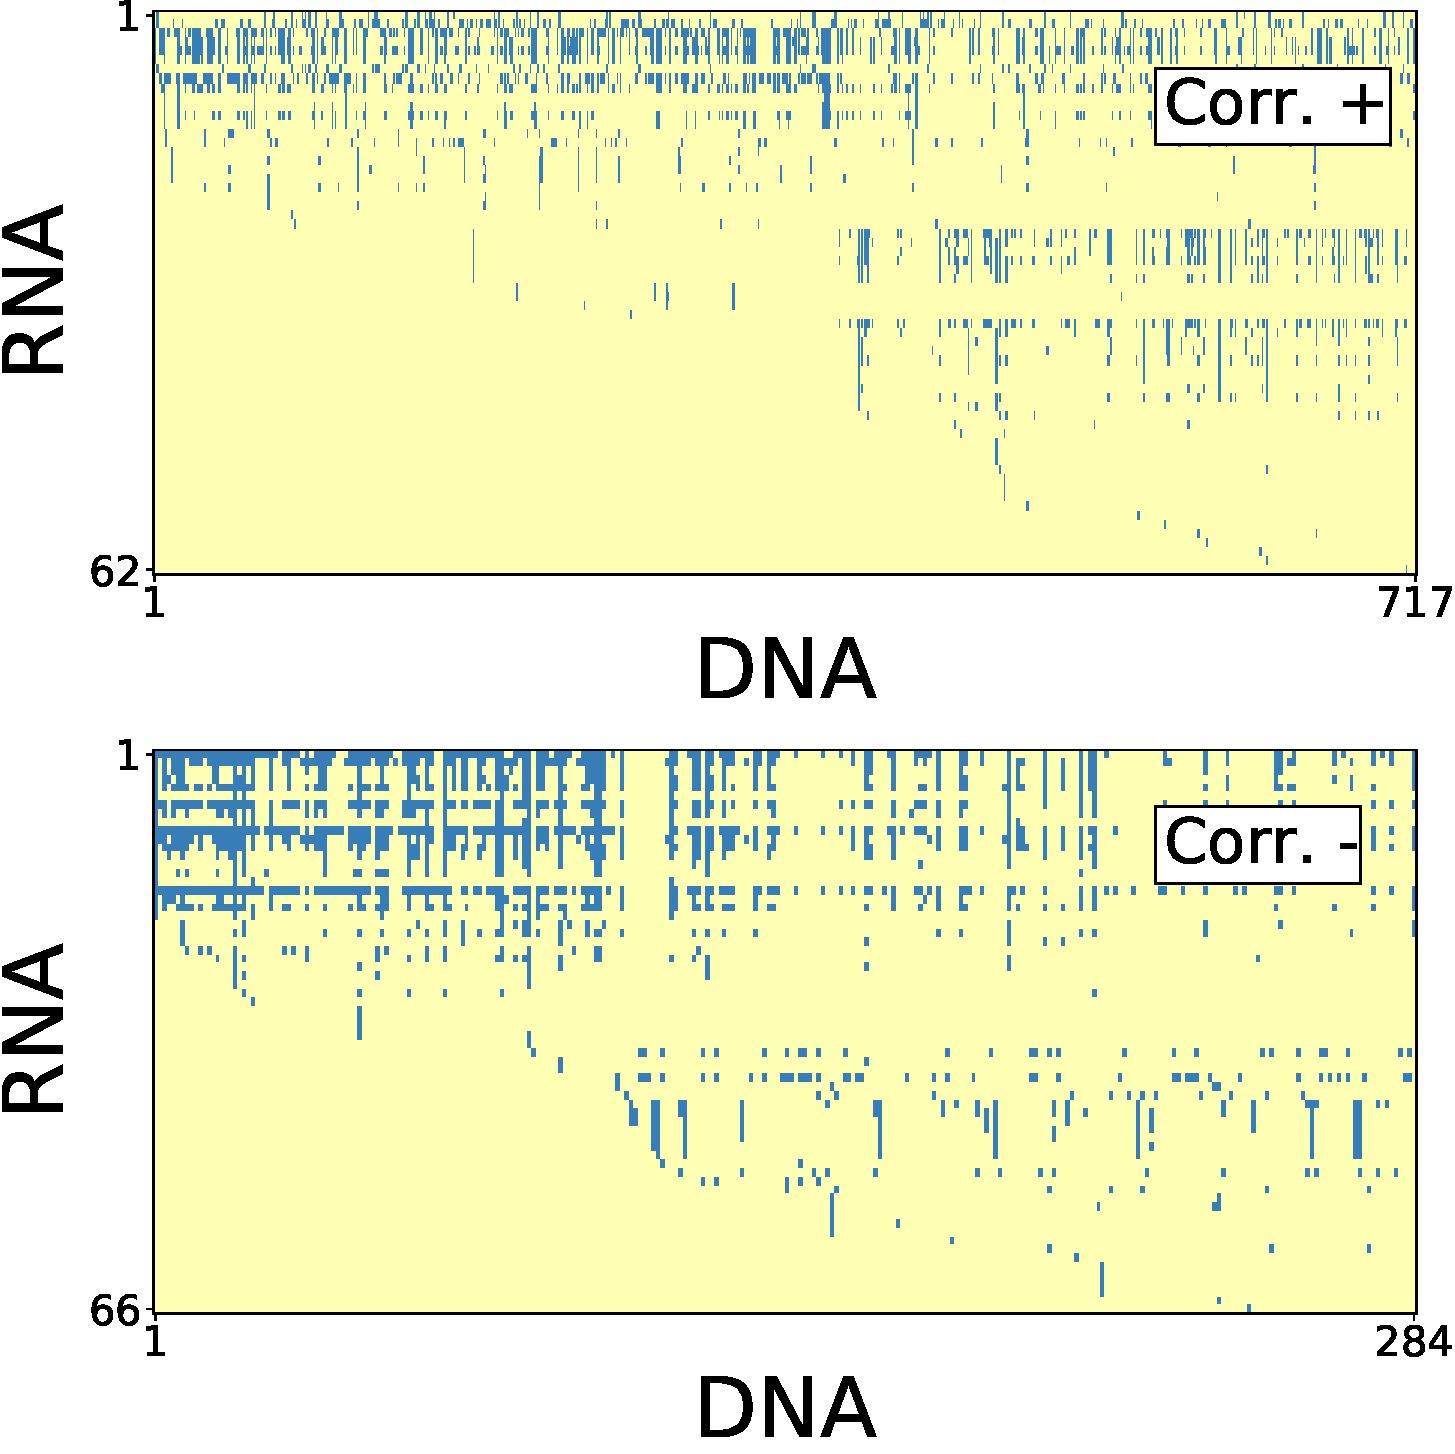
\includegraphics[width=\columnwidth]{FIG/ADN-ARN_Matrix-unit-0.6.pdf}
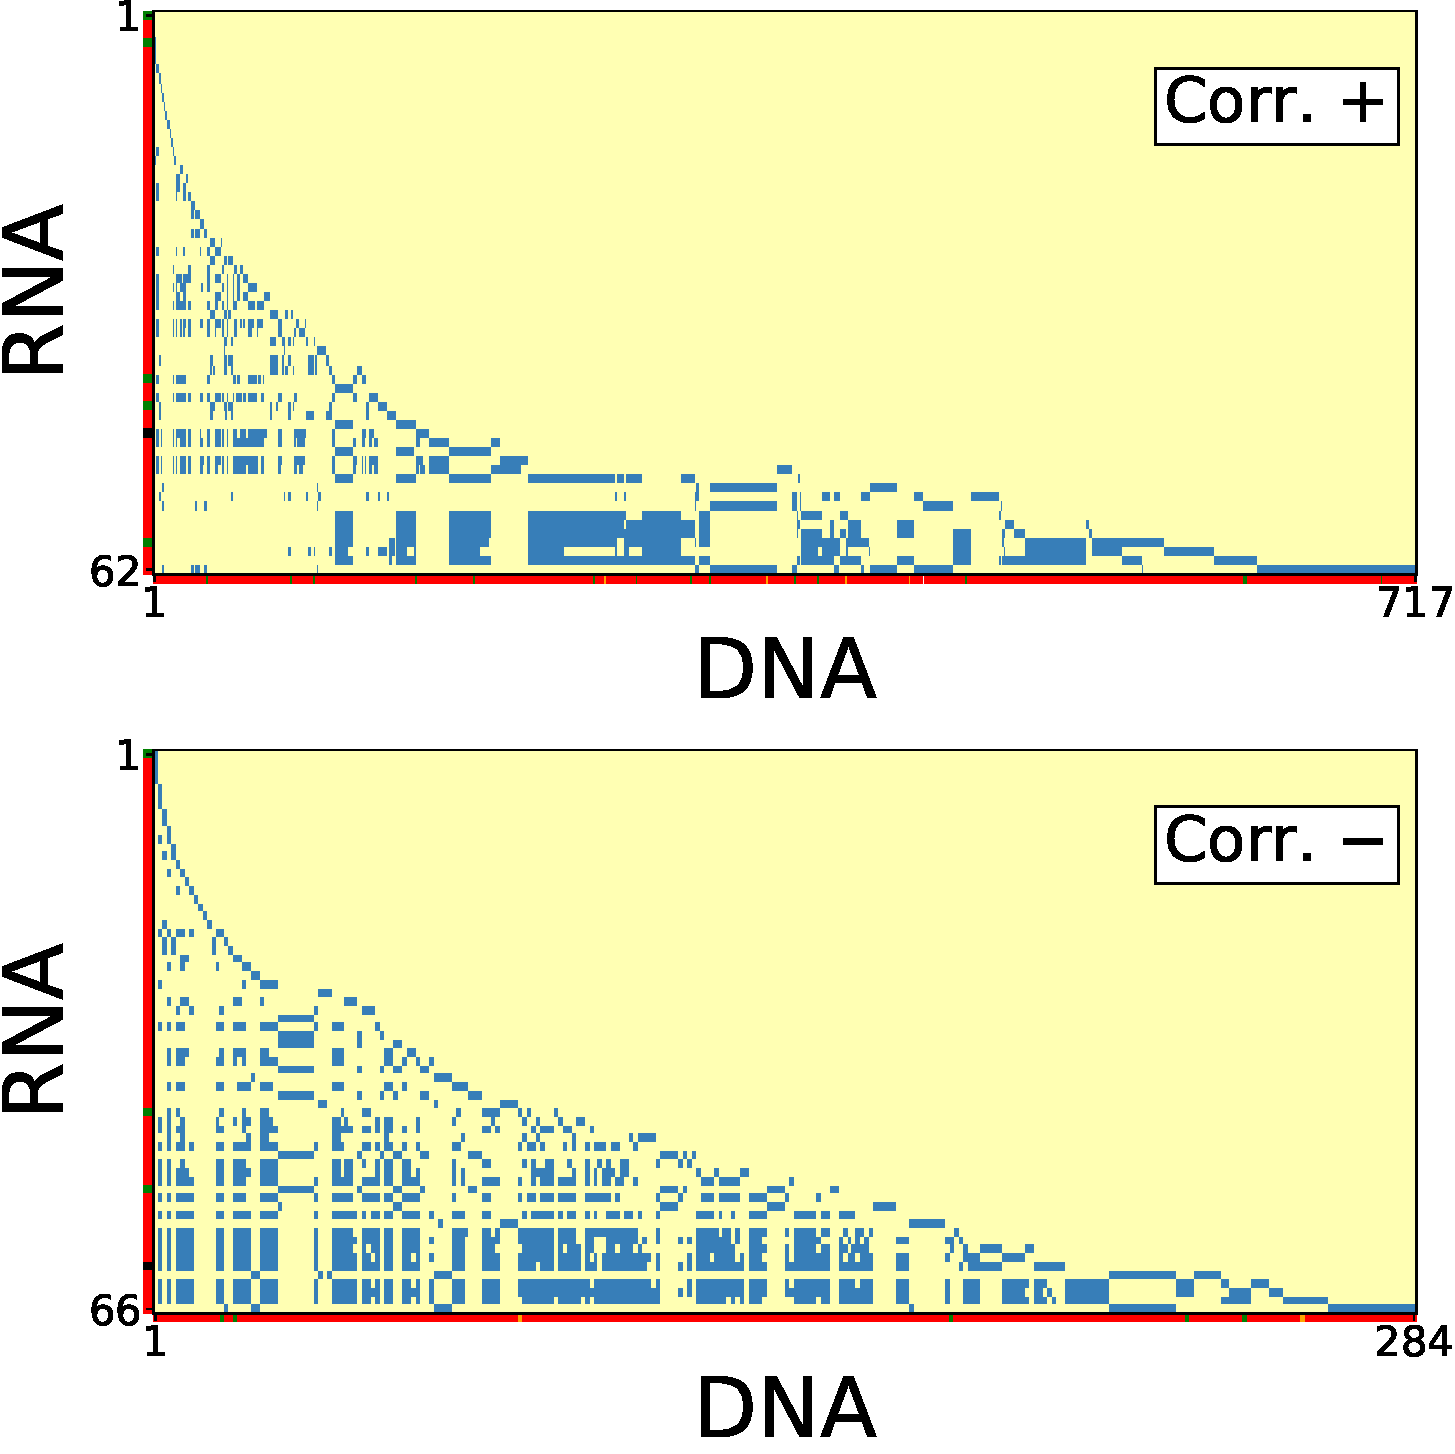
\includegraphics[width=\columnwidth]{FIG/ADN-ARN_FQ-Matrix-sum-unit-0.6.pdf}
}
\begin{center}
\vspace{-2pt}
\rule{\textwidth}{2pt}
\end{center}
\resizebox{\columnwidth}{!}{%
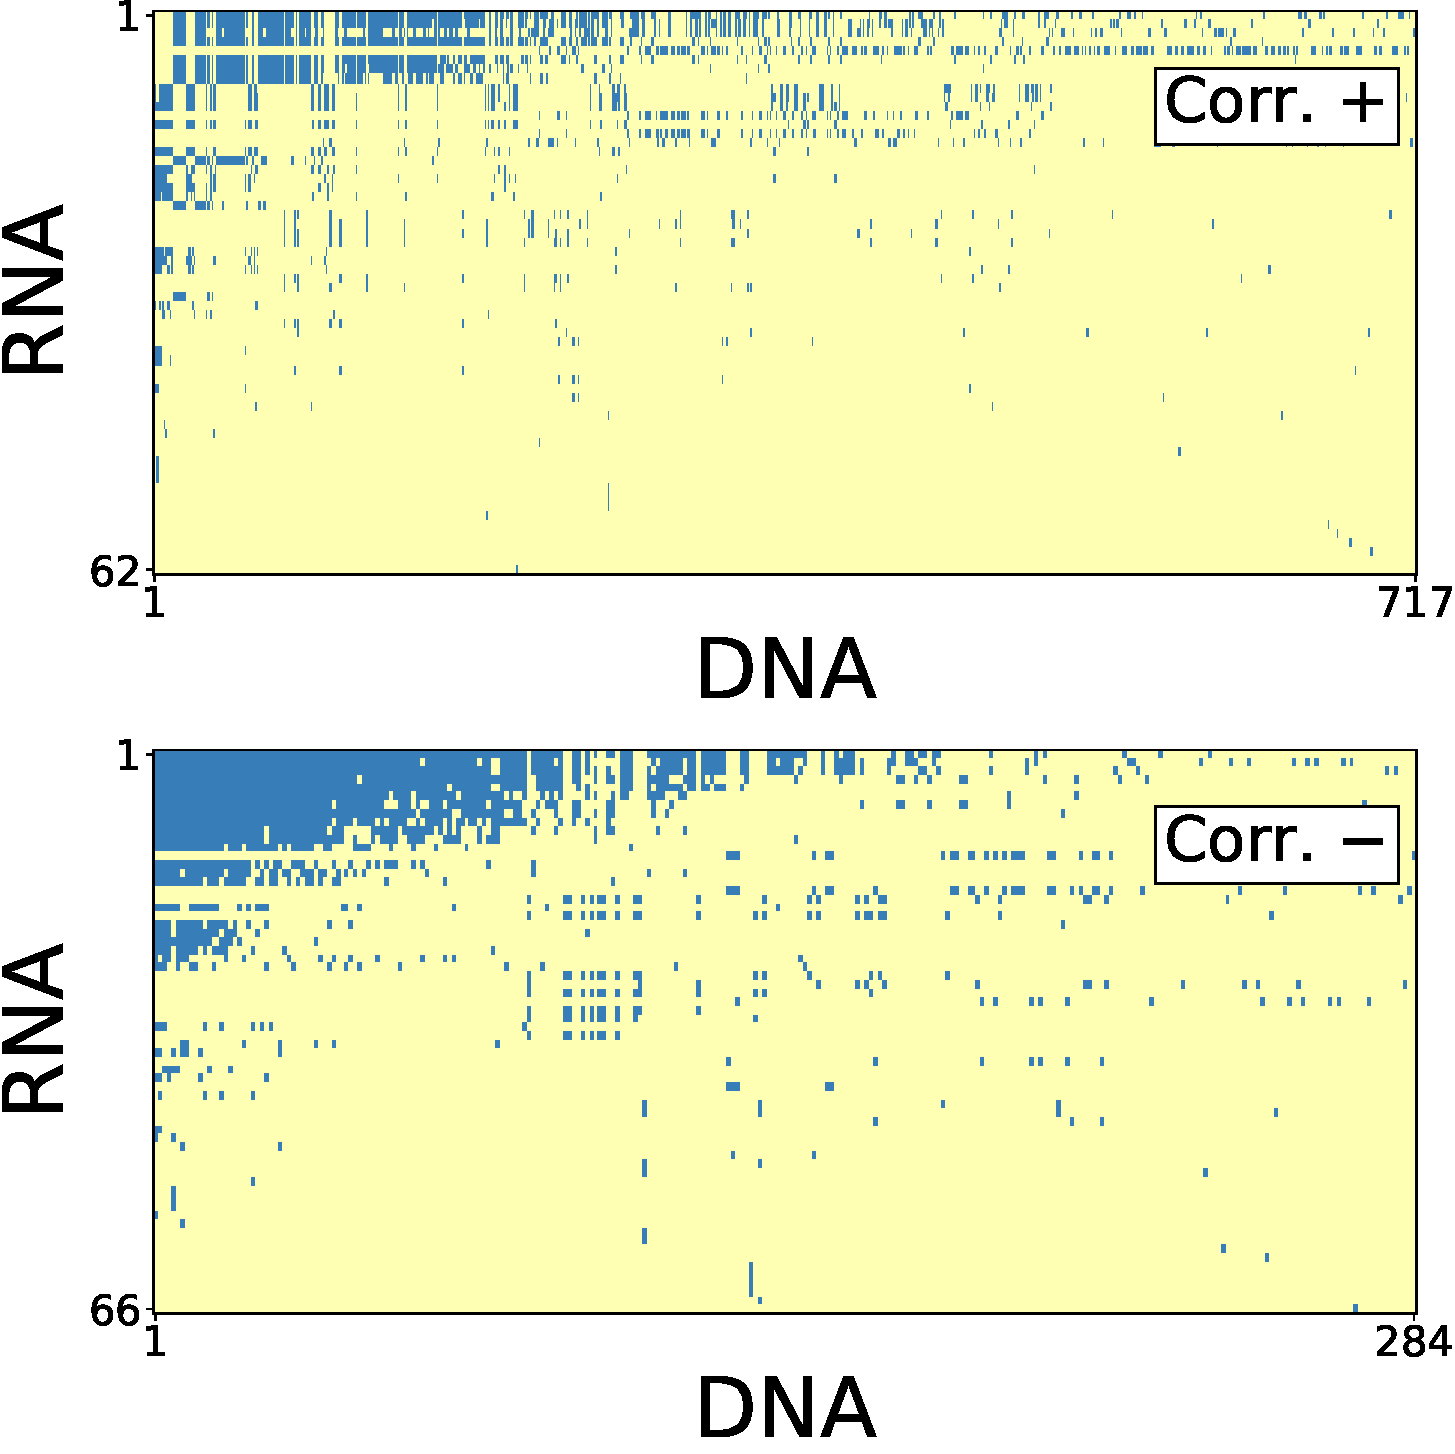
\includegraphics[width=\columnwidth]{FIG/ADN-ARN_Degree-Matrix-unit-0.6.pdf}
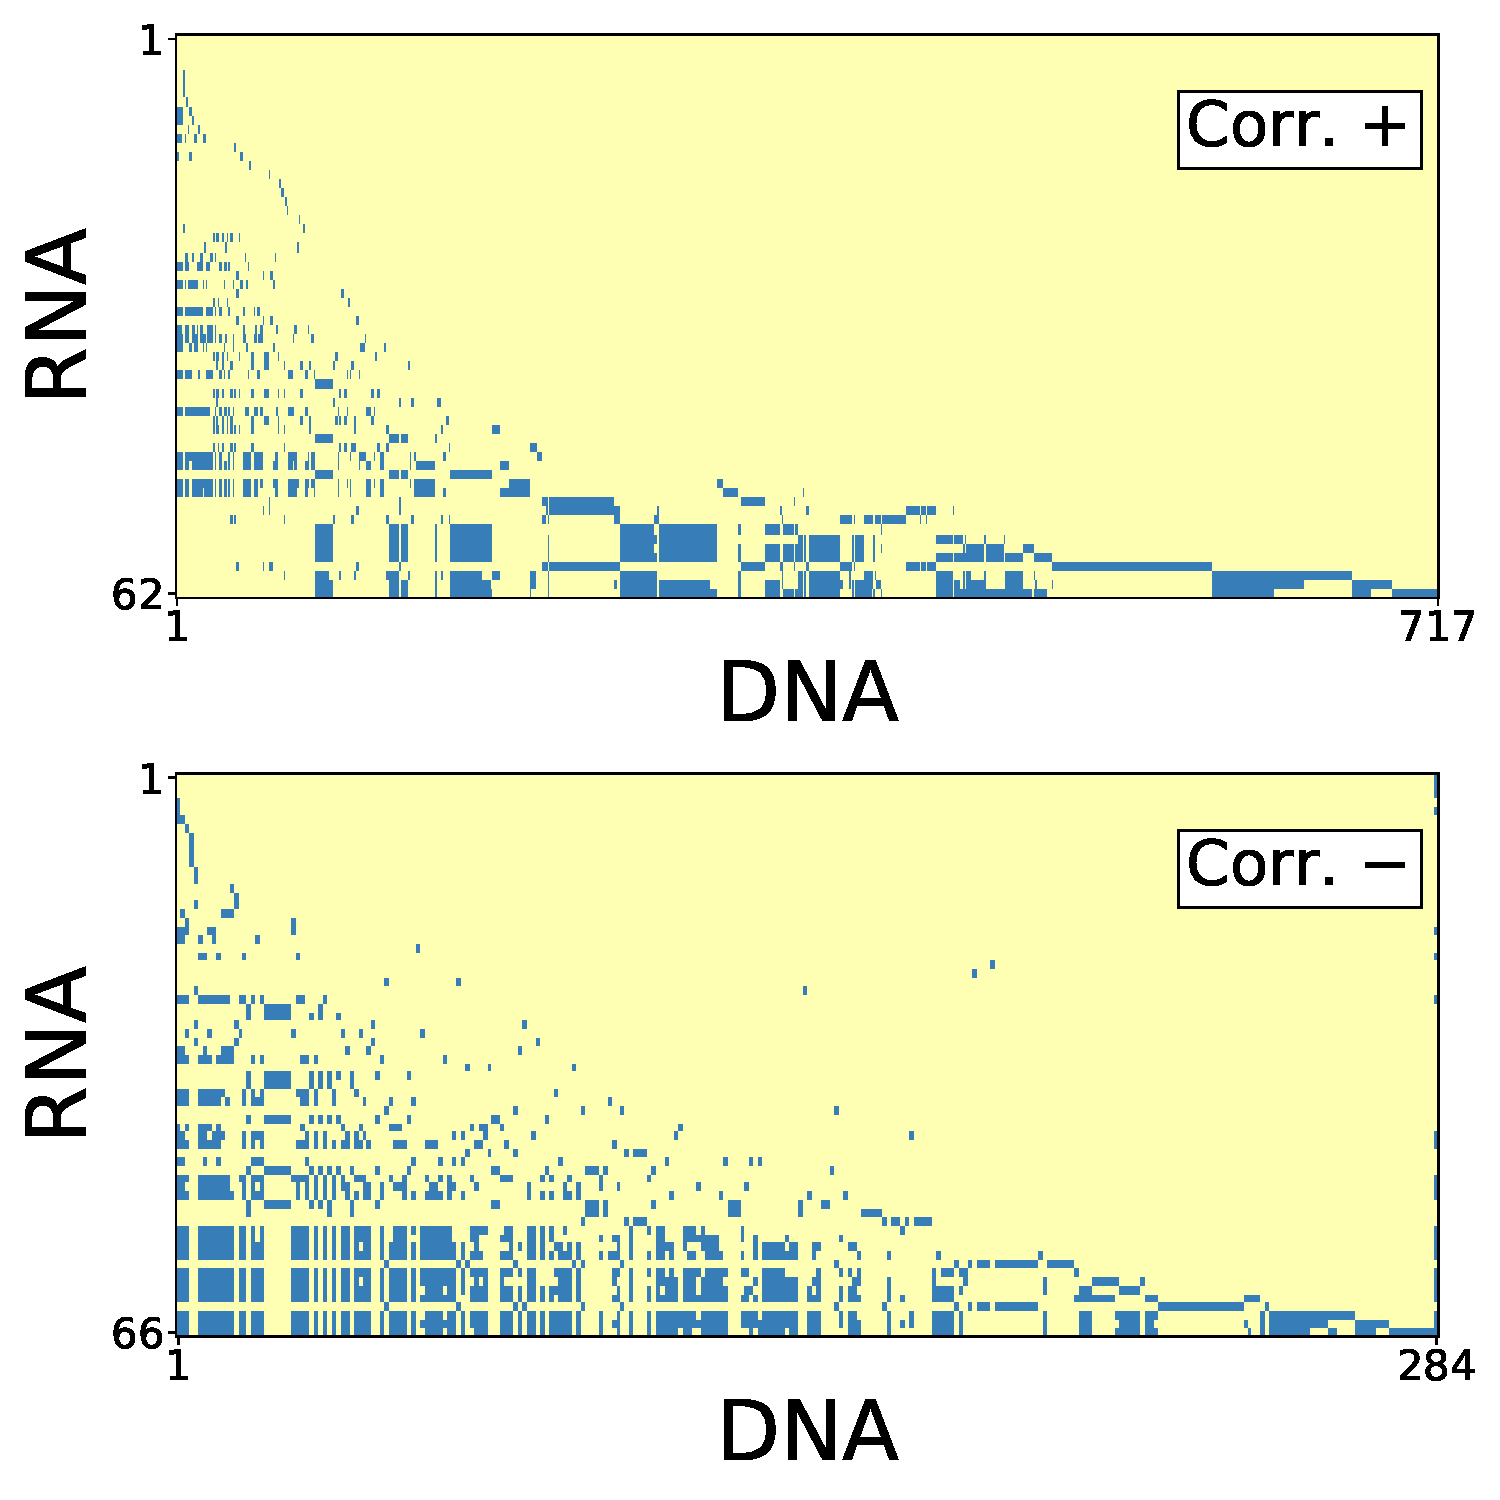
\includegraphics[width=\columnwidth]{FIG/ADN_ARN_BINMATNEST-Matrix-unit-0.6.pdf}
}
\caption{\label{fig:fig2}Binary bi-adjacency matrix representing the interactions between DNAs and RNAs involved in ESR1 synthesis and regulation. Matrix entries equal to $1$ (blue cells) if there is an interaction between entities, $0$ otherwise (bright yellow cells). Raw matrix (top left), Fitness and Complexity based reorganized matrix (top right), Degree based reorganized matrix (bottom left) and matrix reorganized with BINMATNEST algorithm (bottom right). For each panel, two matrices are presented, the one containing positive correlations are at the top, negative correlations are at the bottom. Here we have considered all Pearson correlation such that $|\rho| \geq 0.6$. Color code in the top right panel gives information about CGs and RNAs role. CG of ESR1 is in black, CG (RNA) of ESR1 regulator in green, CG (RNA) of ESR1 regulated in red, orange is for CG being both a ESR1 regulator and regulated and white is for CGs being ESR1's CG, regulator and regulated.}
\end{figure}
 \begin{table}[h!]
\centering
\caption{\label{tab:tab3}Top 10 of the best RNAs and CGs, and their role in ESR1 synthesis and regulation, in terms of Complexity and Fitness score for Positive and negative Pearson correlation coefficients in the context of a threshold $\rho_{c} = 0.6$.}
\begin{tabular}{|ll|ll|ll|ll|}
\cline{1-8}
\multicolumn{4}{|c}{CGs}&\multicolumn{4}{c|}{RNAs}\\
\cline{1-8}
Negative & Role & Positive & Role & Negative & Role & Positive & Role\\
\cline{1-8}
cg22275306 & regulated & cg14534336 & regulated & PPARG & regulator & PR & regulator\\
cg03633268 & regulated & cg17391830 & regulated & HSPB7 & regulated & CAPN8 & regulated\\
cg17391830 & regulated & cg22761619 & regulated & KCNIP2 & regulated & LONRF2 & regulated\\
cg03228065 & regulated & cg10216820 & regulated & ITGA7 & regulated & FOXM1 & regulator\\
cg27647589 & regulated & cg20631750 & regulated & CAPN8 & regulated & BIRC5 & regulated\\
cg02385230 & regulated & cg05539265 & regulated & SYTL5 & regulated & NUF2 & regulated\\
cg03190578 & regulated & cg03451296 & regulated & UBXN10 & regulated & TFF1 & regulated\\
cg03387103 & regulated & cg20284025 & regulated & FAM13C & regulated & FAM13C & regulated\\
cg11938491 & regulated & cg18263686 & regulated & IGF1 & regulated & ZG16B & regulated\\
cg14843902 & regulated & cg24282422 & regulated & SCNN1A & regulated & MGAM2 & regulated\\
\cline{1-8}
\end{tabular}
\end{table}
 \begin{table}[h!]
\centering
\caption{\label{tab:tab4}Top 10 of the worst RNAs and CGs, and their role in ESR1 synthesis and regulation, in terms of Complexity and Fitness score for Positive and negative Pearson correlation coefficients in the context of a threshold $\rho_{c} = 0.6$.}
\begin{tabular}{|ll|ll|ll|ll|}
\cline{1-8}
\multicolumn{4}{|c}{CGs}&\multicolumn{4}{c|}{RNAs}\\
\cline{1-8}
Negative & Role & Positive & Role & Negative & Role & Positive & Role\\
\cline{1-8}
cg25296982 & regulated & cg22512377 & regulated & MID1 & regulated & MID1 & regulated\\
cg25316898 & regulated & cg18664900 & regulated & PRR15 & regulated & SIT1 & regulated\\
cg18006085 & regulated & cg27168900 & regulated & MLPH & regulated & BANK1 & regulated\\
cg22356484 & regulated & cg18439323 & regulated & FOXA1 & regulated & IRF4 & regulator\\
cg26833538 & regulated & cg19561609 & regulated & ID4 & regulated & CCR7 & regulated\\
cg24317002 & regulated & cg20889476 & regulated & ESR1 & & ICOS & regulated\\
cg24845324 & regulated & cg20074699 & regulated & TTC6 & regulated & GZMM & regulated\\
cg23859078 & regulated & cg26572856 & regulated & C5AR2 & regulated & BBOX1 & regulated\\
cg24775832 & regulated & cg19897251 & regulated & CA12 & regulated & PPP2R2B & regulated\\
cg26550787 & regulated & cg20803232 & regulated & AGR3 & regulated & ID4 & regulated\\
\cline{1-8}
\end{tabular}
\end{table}
\begin{figure}[h!]
\resizebox{\columnwidth}{!}{%
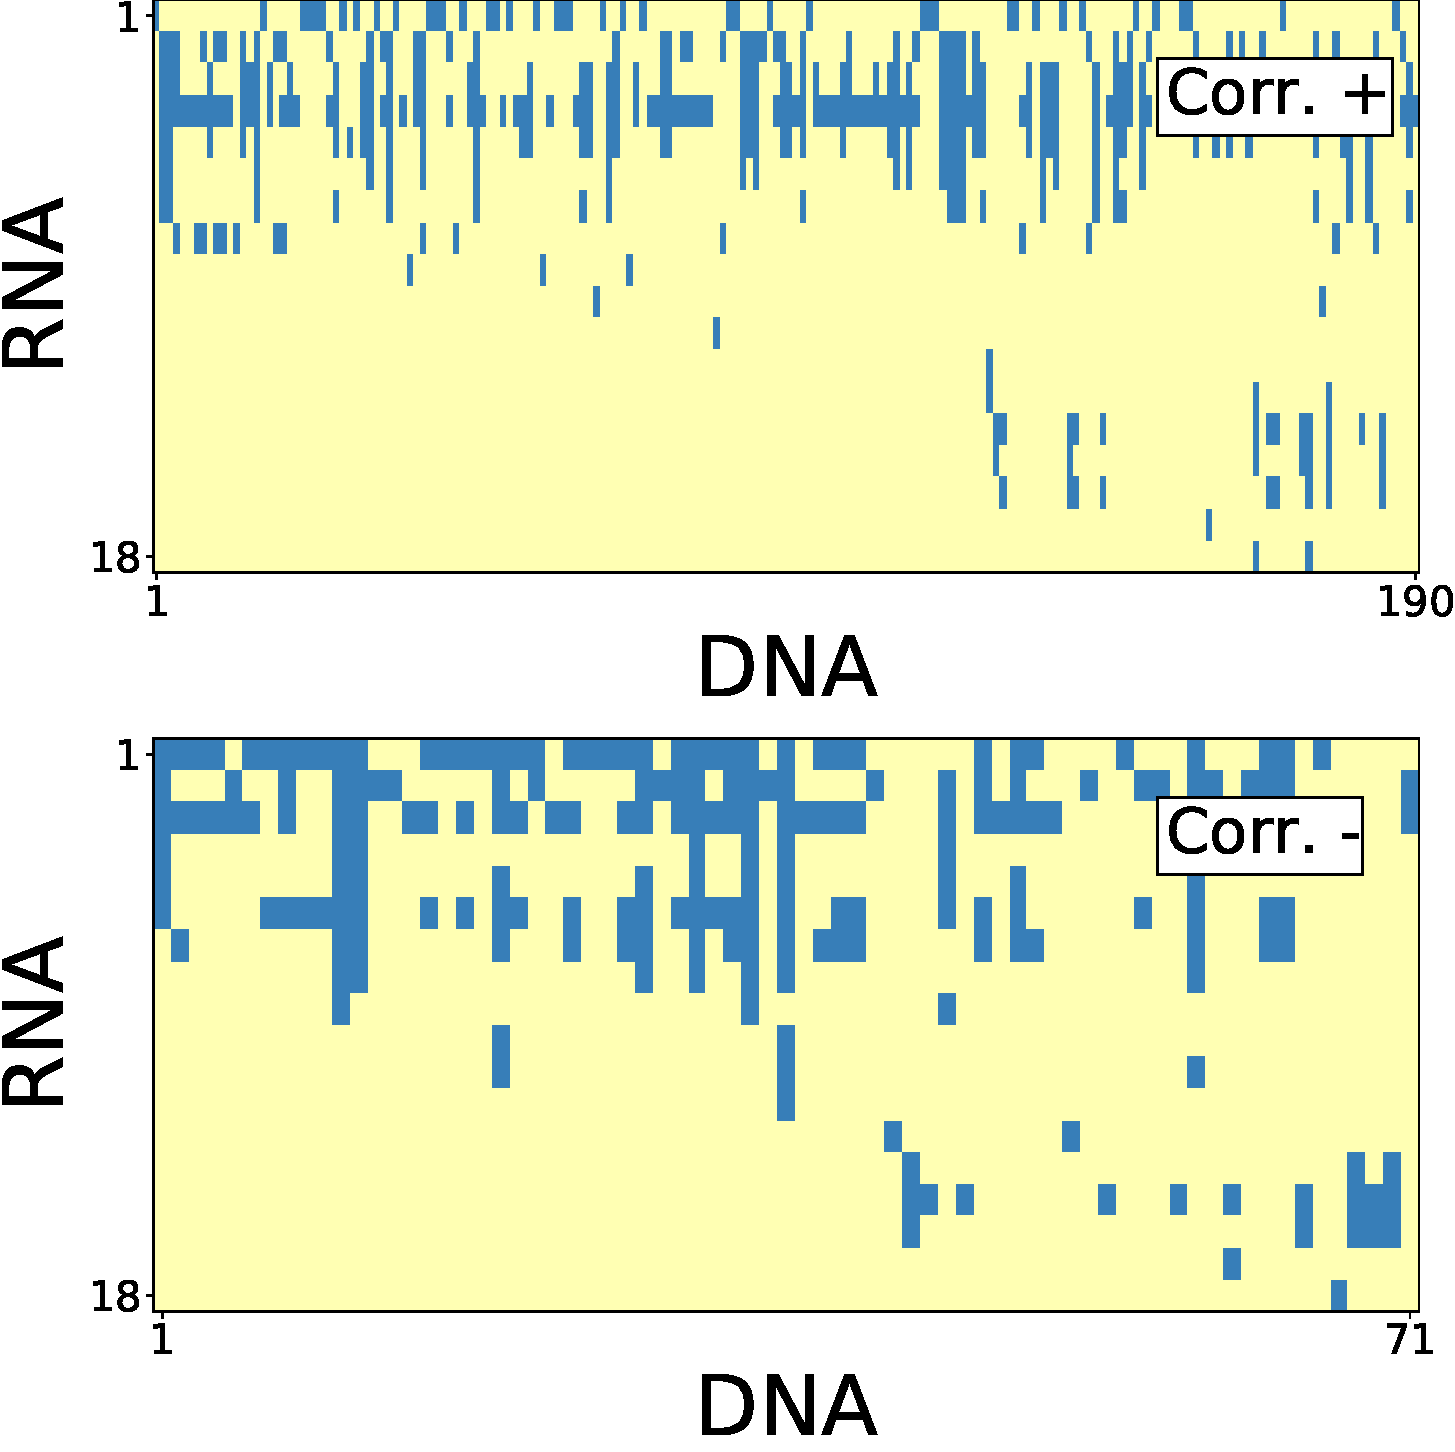
\includegraphics[width=\columnwidth]{FIG/ADN-ARN_Matrix-unit-0.7.pdf}
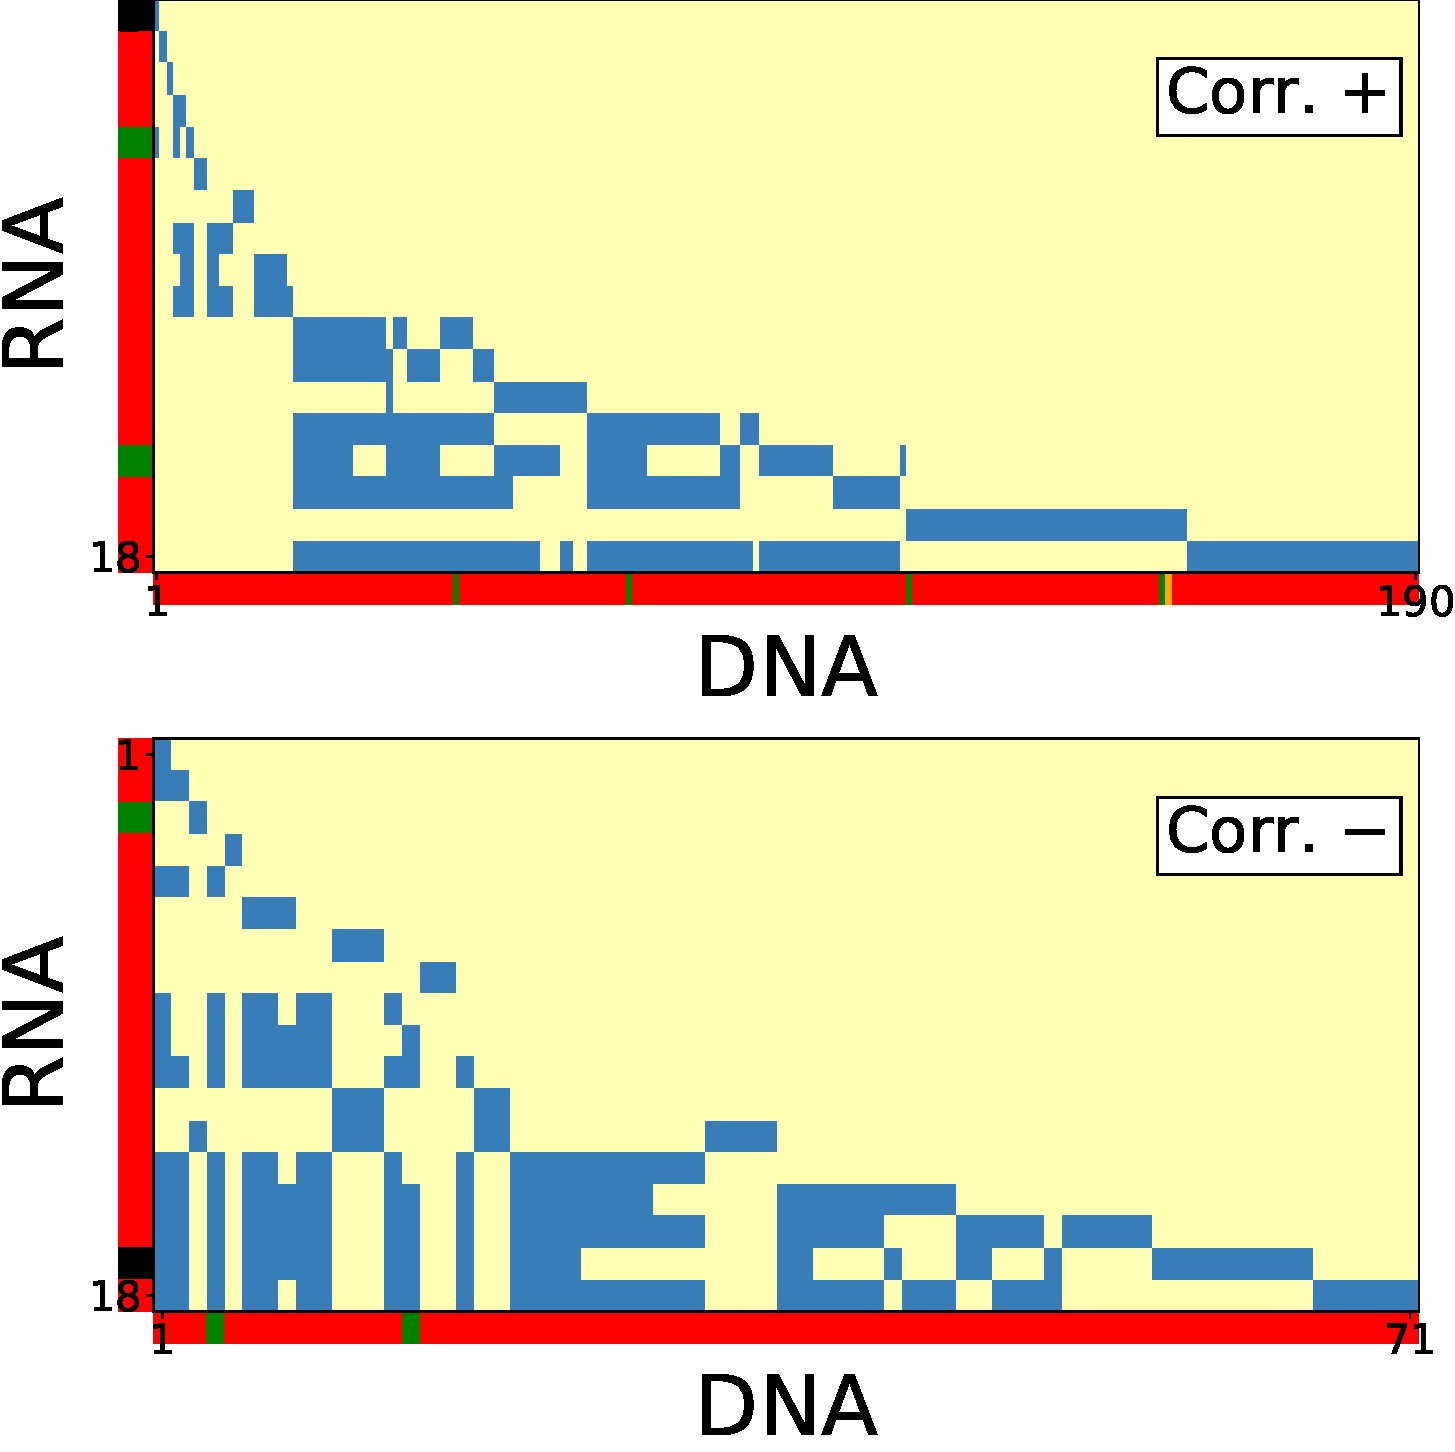
\includegraphics[width=\columnwidth]{FIG/ADN-ARN_FQ-Matrix-sum-unit-0.7.pdf}
}
\begin{center}
\vspace{-2pt}
\rule{\textwidth}{2pt}
\end{center}
\resizebox{\columnwidth}{!}{%
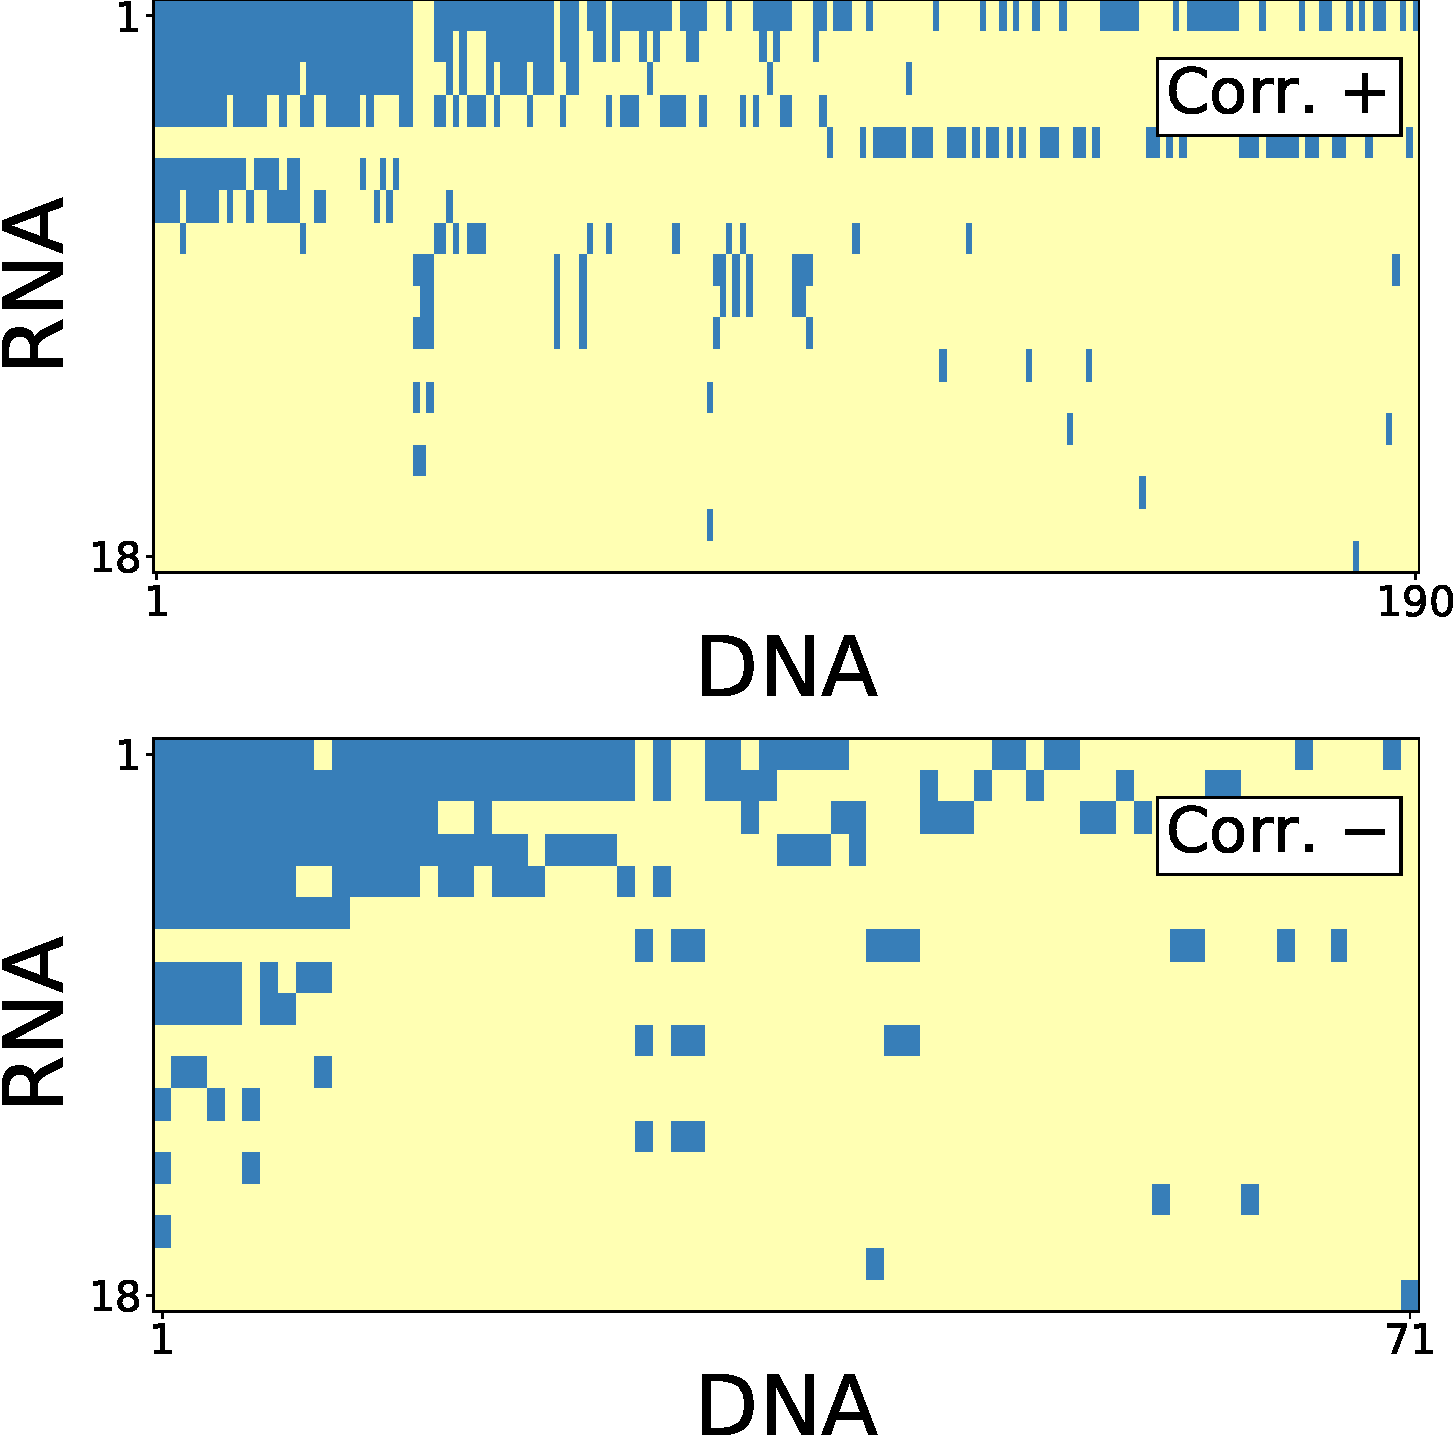
\includegraphics[width=\columnwidth]{FIG/ADN-ARN_Degree-Matrix-unit-0.7.pdf}
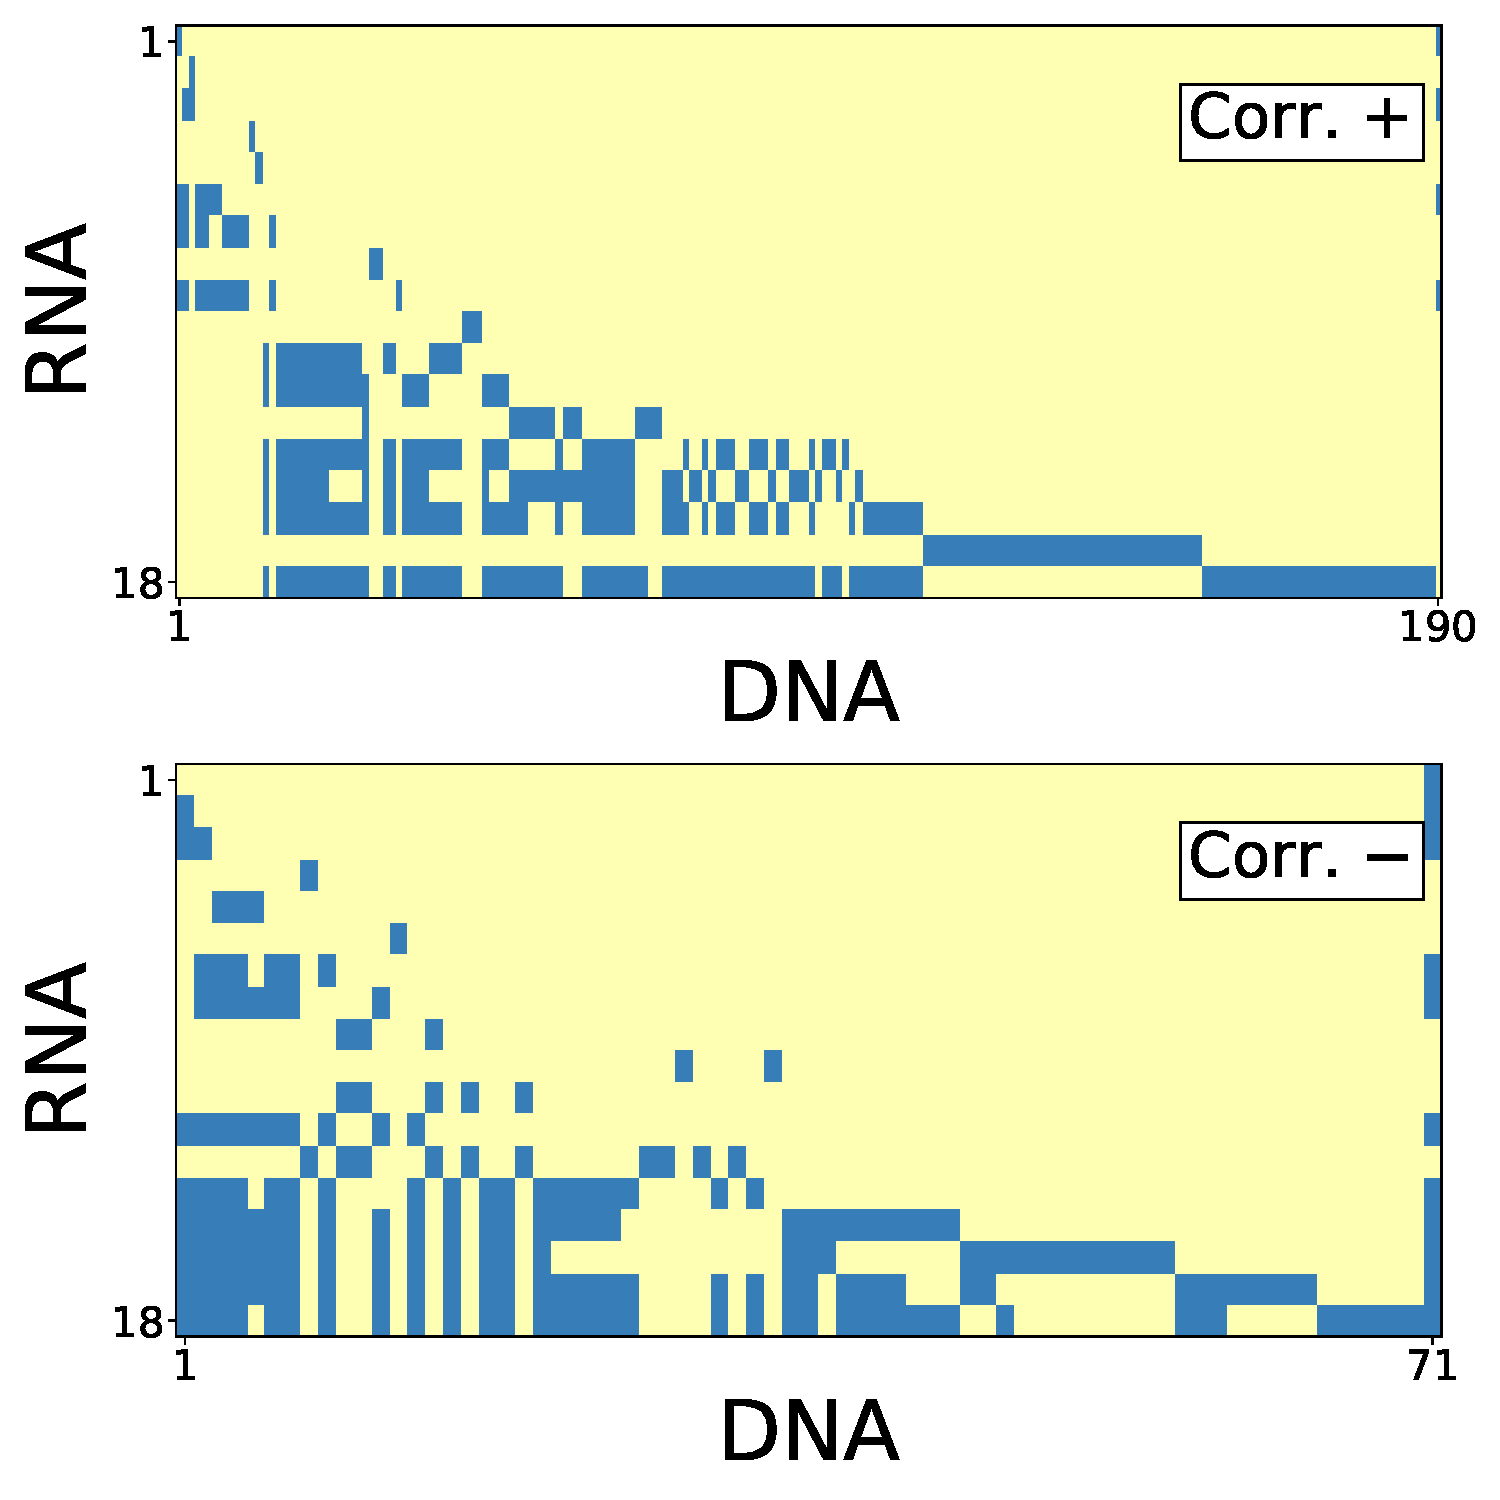
\includegraphics[width=\columnwidth]{FIG/ADN_ARN_BINMATNEST-Matrix-unit-0.7.pdf}
}
\caption{\label{fig:fig3}Binary bi-adjacency matrix representing the interactions between DNAs and RNAs involved in ESR1 synthesis and regulation. Matrix entries equal to $1$ (blue cells) if there is an interaction between entities, $0$ otherwise (bright yellow cells). Raw matrix (top left), Fitness and Complexity based reorganized matrix (top right), Degree based reorganized matrix (bottom left) and matrix reorganized with BINMATNEST algorithm (bottom right). For each panel, two matrices are presented, the one containing positive correlations are at the top, negative correlations are at the bottom. Here we have considered all Pearson correlation such that $|\rho| \geq 0.7$. Color code in the top right panel gives information about CGs and RNAs role. CG of ESR1 is in black, CG (RNA) of ESR1 regulator in green, CG (RNA) of ESR1 regulated in red, orange is for CG being both a ESR1 regulator and regulated and white is for CGs being ESR1's CG, regulator and regulated.}
\end{figure}
 \begin{table}[h!]
\centering
\caption{\label{tab:tab5}Top 10 of the best RNAs and CGs, and their role in ESR1 synthesis and regulation, in terms of Complexity and Fitness score for Positive and negative Pearson correlation coefficients in the context of a threshold $\rho_{c} = 0.7$.}
\begin{tabular}{|ll|ll|ll|ll|}
\cline{1-8}
\multicolumn{4}{|c}{CGs}&\multicolumn{4}{c|}{RNAs}\\
\cline{1-8}
Negative & Role & Positive & Role & Negative & Role & Positive & Role\\
\cline{1-8}
cg02385230 & regulated & cg11694119 & regulated & TFF3 & regulated & ESR1 & \\
cg03633268 & regulated & cg03451296 & regulated & CT62 & regulated & APOA4 & regulated\\
cg24546153 & regulated & cg20284025 & regulated & IRF4 & regulator & CBFA2T3 & regulated\\
cg20078972 & regulator & cg24183909 & regulated & TSPAN1 & regulated & TTC6 & regulated\\
cg19321739 & regulated & cg22761619 & regulated & THSD4 & regulated & AR & regulator\\
cg03190578 & regulated & cg23784313 & regulated & FSIP1 & regulated & ID4 & regulated\\
cg03228065 & regulated & cg07052041 & regulated & CCR7 & regulated & PTH1R & regulated\\
cg16013349 & regulated & cg22877623 & regulated & ID4 & regulated & MLPH & regulated\\
cg02212575 & regulated & cg10617287 & regulated & CA12 & regulated & PRR15 & regulated\\
cg02711212 & regulated & cg18006085 & regulated & C5AR2 & regulated & FOXA1 & regulated\\
\cline{1-8}
\end{tabular}
\end{table}
 \begin{table}[h!]
\centering
\caption{\label{tab:tab6}Top 10 of the worst RNAs and CGs, and their role in ESR1 synthesis and regulation, in terms of Complexity and Fitness score for Positive and negative Pearson correlation coefficients in the context of a threshold $\rho_{c} = 0.7$.}
\begin{tabular}{|ll|ll|ll|ll|}
\cline{1-8}
\multicolumn{4}{|c}{CGs}&\multicolumn{4}{c|}{RNAs}\\
\cline{1-8}
Negative & Role & Positive & Role & Negative & Role & Positive & Role\\
\cline{1-8}
cg18623708 & regulated & cg24751886 & regulated & FOXA1 & regulated & SIT1 & regulated\\
cg16773127 & regulated & cg17826679 & regulated & ESR1 & & MID1 & regulated\\
cg02477603 & regulated & cg24704593 & regulated & MLPH & regulated & CCR7 & regulated\\
cg01099300 & regulated & cg21038780 & regulated & PRR15 & regulated & IRF4 & regulator\\
cg03995434 & regulated & cg21210531 & regulated & TTC6 & regulated & ICOS & regulated\\
cg05089968 & regulated & cg23543604 & regulated & SIT1 & regulated & BANK1 & regulated\\
cg18263686 & regulated & cg13556253 & regulated & ICOS & regulated & GZMM & regulated\\
cg18174678 & regulated & cg10444350 & regulated & AGR3 & regulated & CXCL9 & regulated\\
cg15043801 & regulated & cg12737152 & regulated & C5AR2 & regulated & FOXA1 & regulated\\
cg11938491 & regulated & cg00952322 & regulated & CA12 & regulated & PRR15 & regulated\\
\cline{1-8}
\end{tabular}
\end{table}
 \begin{table}[h!]
\centering
\caption{\label{tab:tab1}Nestedness scores of the network. The NODF (BINMATNEST) score goes from $0$ ($100$) for non nested network to $1$ ($0$) for highly nested network. For each threshold, the table gives the scores associated to positive-correlation- and negative-correlation-based networks, annotated - and + respectively.}
\begin{tabular}{|l|l|l|l|l|}
\cline{1-5}
\multirow{2}{*}{Threshold} & \multicolumn{2}{c|}{NODF} & \multicolumn{2}{c|}{BINMATNEST}\\
\cline{2-5}
&-&+&-&+\\
\cline{1-5}
0.5 & 0.22 & 0.24 & 1.6 & 1.3\\
0.6 & 0.34 & 0.24 & 2.4 & 1.6 \\
0.7 & 0.46 & 0.46 & 5 & 3.3\\
\cline{1-5}
\end{tabular}
\end{table}
\clearpage
\printbibliography
	\end{document}